\documentclass{article}
\usepackage{color}
\usepackage{amsmath}
\usepackage{graphicx}
\usepackage{tgtermes}
\usepackage{forest}
\usepackage{fancyvrb}
\usepackage{setspace}
\usepackage[font=small,labelfont=bf]{caption}

\forestset{
  tt/.style={
    for tree={
      parent anchor=south,
      child anchor=north,
      grow=270,
      align=center,
      inner sep=0pt
    }
  },
  nice empty nodes up/.style={
    for tree={calign=fixed edge angles},
    delay={where content={}{shape=coordinate,for parent={for children={anchor=south}}}{}}
  }
}
\begin{document}
\title{\textbf{AI assistants}: A framework for semi-automated, transparent, tooling-rich data wrangling}
\author{Tomas Petricek}
\maketitle
% \begin{abstract}
%   zz
% \end{abstract}

\newcommand{\ident}[1]{\textnormal{\sffamily #1}}
\definecolor{tpclr}{rgb}{0.6,0,0.3}
\newcommand{\tpnote}[1]{{\marginpar{
  \setstretch{0.8}\raggedright\textcolor{tpclr}{ \footnotesize{\textbf{Tomas:} #1 } }}
}}
~

\section{Introduction}
\tpnote{This part is written as an intro to a potential paper about AI assistants 
(using many ideas and formulations from Charles et al.)}

According to some reports, 80\% of data analysis is spent on \emph{data wrangling} -- an activity
that encompasses obtaining data from a diversity of semi-structured sources, making sense of data
encoding, joining multiple datasets with mismatched structure, correcting erroneous records and 
filling missing data. Despite the recent rise of artificial intelligence and machine learning, 
data wrangling has, so far, largely eluded automation and remains a tedious and time-consuming 
manual task.

There are a number of reasons why data wrangling is hard to automate. First, data is often big and 
diverse and hide hard-to-find special cases that can be only handled with some human insight.
Second, real-world data is heterogeneous. Automatic methods developed for one kind of data will 
often fail when more data is added. Third, data cleaning often requires tuning of many parameters 
and you often cannot know what will work until you review the results. Finally, making an error
during data wrangling can have a disasterous effect on a project. An automatic tool can easily 
confuse interesting outliers for an uninteresting noise in cases where a quick human glance would
immediately spot the distinction.

For these rasons, we argue that a major advance in data wrangling is best achieved by developing
semi-automatic methods that allow us to effectively combine automation and scalability of machine 
learning methods with human insight. To capture the human-computer interaction pattern that is
required for data wrangling, we introduce the concept of an \emph{AI assistant}. An AI assistant
is a component that interacts with a data analyst to guide them through a single data extraction,
collection, integration, preparation or exploration task. AI assistants are semi-automated, 
transparent and tooling-rich:
%
\begin{enumerate}
\item \textbf{Semi-automated.} After being invoked on input data, the AI assistant runs some automated
  data wrangling algorithm (based on AI, machine learning or statistical analysis) and offers a list
  of suggestions to the data analyst. The analyst can review the results, choose one of the provided
  options or, more generally, provide feedback back to the algorithm. The loop is repeated until 
  the AI assistant has no further suggestions or until the analyst accepts one of the suggested results.

\vspace{-0.2em}
\item \textbf{Transparent.} An AI assistant needs to explain what cleaning operations it recommends. 
  At each step, the result of running an AI assistant is a short data wrangling script, written 
  in a domain-specific language, designed for each individual assistant. The data analyst can 
  review the script to assess if the recommended cleaning operation is reasonable, before running
  the script on the input data.
  
\vspace{-0.2em}
\item \textbf{Tooling-rich.} Finally, an AI assistant needs to play well with modern data science
  tooling. This means that offering the suggestions to the data analyst should be done through an 
  interactive programming mechanism such as auto-complete. When reviewing suggestions, the data 
  analyst should also immediately see a preview of running the script on the actual input data as,
  for example, when running code in Jupyter notebooks.
\end{enumerate}
%
Several tools that satisfy the above definition of an AI assistant have been built in the past, 
but our main motivation is to describe the general structure of an AI assistant abstractly and
discuss the methodology of developing and evaluating AI assistants.

A data analyst will typically need to interact with many separate assistants over the course of an
anlysis, each of which specializes in a single kind of task. Having a clear abstract definition
of what an AI assistant is, together with several examples, will provide a common framework that 
developers of AI assistants and authors of data science tools can use in order to build a 
flourishing ecosystem for semi-automated, transparent, tooling-rich data wrangling.

\tpnote{I think this is good structure of contributions for a real paper. The current version does not quite do all this yet though!}
This paper explains what an AI assistant is, discusses how it can be integrated in a notebook
environment for data science and gives a number of examples of AI assistants: 
%
\begin{itemize}
\item We give a formal description that models AI assistants as trees (Section~\ref{sec:trees}). 
  An AI assistant offers user a choice by generating multiple sub-trees and the user makes a choice 
  and provides an input to the AI assistant by choosing one branch.
\vspace{-0.2em}
\item We discuss the integration of AI assistants in the Wrattler notebook system (Section~\ref{sec:notebook}). 
  This makes it easy to use AI assistants interactively and Wrattler also gives rapid feedback when 
  cleaning data using an AI assistant. 
\vspace{-0.2em}
\item We give two examples of AI assistants and explain how the tree-based model captures those
  examples (Section~\ref{sec:examples}). We consider \emph{Datadiff}, which automates the process of reconcilling 
  inconsistencies between pairs of tabular data sets and a \emph{CSV parser} that extracts typed
  data from real-world messy CSV files.
\vspace{-0.2em}
\item We consider two ways of evaluating AI assistants (Section~\ref{sec:evaluation}). An AI 
  assistant should provide the best answer when used fully automatically, but user interaction 
  should allow correcting it when the answer obtained automatically is not right.
\end{itemize}

\section{Background}
\label{sec:background}
\tpnote{These are comments for AIDA team readers only, somewhat overlapping with the introduction.
We'll need to rewrite this for a real paper. }

The idea of an \emph{AI assistant} appeared in many contexts in the AIDA project.
Wrattler aims to provide a platform through which AI assistants can be 
easily used; the datadiff project developed an AI assistant which automates the process of 
reconciling inconsistencies between pairs of tabular datasets. However, we never clearly defined
what an AI assistant is. 

A simple way of trying to address the data wrangling problem would be to build a set of functions
that take some dirty datasets and produce one or more clean datasets. The user could then call these
functions on their dirty data and would get a clean result. The function would likely take some
parameters that specify how cleaning should be done. (Conceivably, this could be further automated
and a system could invoke such functions automatically.)

However, this simple approach has two problems. First, real-world data sets often 
contain numerous corner cases that require some human insight and so getting the right results 
might involve laborious fiddling with function parameters. Second, we want the data analysis
to be transparent and be able to understand how have the data wrangling problems been solved. 
A simple function does not address these because it does not encourage human interaction
and it is not transparent -- it produces a result without indicating how and why.

\subsection{Why are assistants more than functions}

\tpnote{I like the idea of contrasting `cleaning function' with an `assistant' but this text
repeats ideas from the intrduction and does not do a very good job overall.}
AI assistants address the above issues. First, AI assistants are interactive. Given 
some data, they perform some analysis and provide the user with several options to choose 
from (those can be most likely solutions to some problem, possible ways of resolving ambiguous
corner cases, or a choice of next steps the AI assistant can follow). In this paper, the options are 
a finite list (where the user has to choose one), but they could also be open-ended (where the user 
can specify some input). The list of options is also sorted by quality (if we always choose the 
most likely option, the assistant will behave as an automatic function).

Second, AI assistants do not directly transform data, but instead, generate scripts (or, more 
formally, expressions) in simple languages (domain-specific languages, or DSLs) that define how 
data should be transformed. The AI assistant can still use sophisticated machine learning 
algorithms (that do not produce an explanation of how they work) behind the scenes, but the end
result will always be a simple script that can be reviewed and understood by the user.

Note that each AI assistant can use its own domain-specific language -- the language should be
as small as possible, i.e. it should be able to express the data transformations that the AI
assistant can recommend, but nothing more. The combination of interactivity and domain-specific 
languages allows us to do a number of interesting things:

\begin{itemize}
\item Scripts generated by AI assistant can be translated to R or Python (and it is easy to 
  add support for other languages), which means that one can use an AI assistant during data
  analysis and exploration, but then end up with code that can be used in production in any
  programming language.

\item The interactive nature of AI assistants makes it possible to give immediate feedback to
  users and let them correct potential issues early. For example, in Wrattler, we display the
  options that AI assistant provides together with a preview of results (of applying the
  generated expression to a sample dataset). 
\end{itemize}

\begin{figure}
\vspace{-1em}
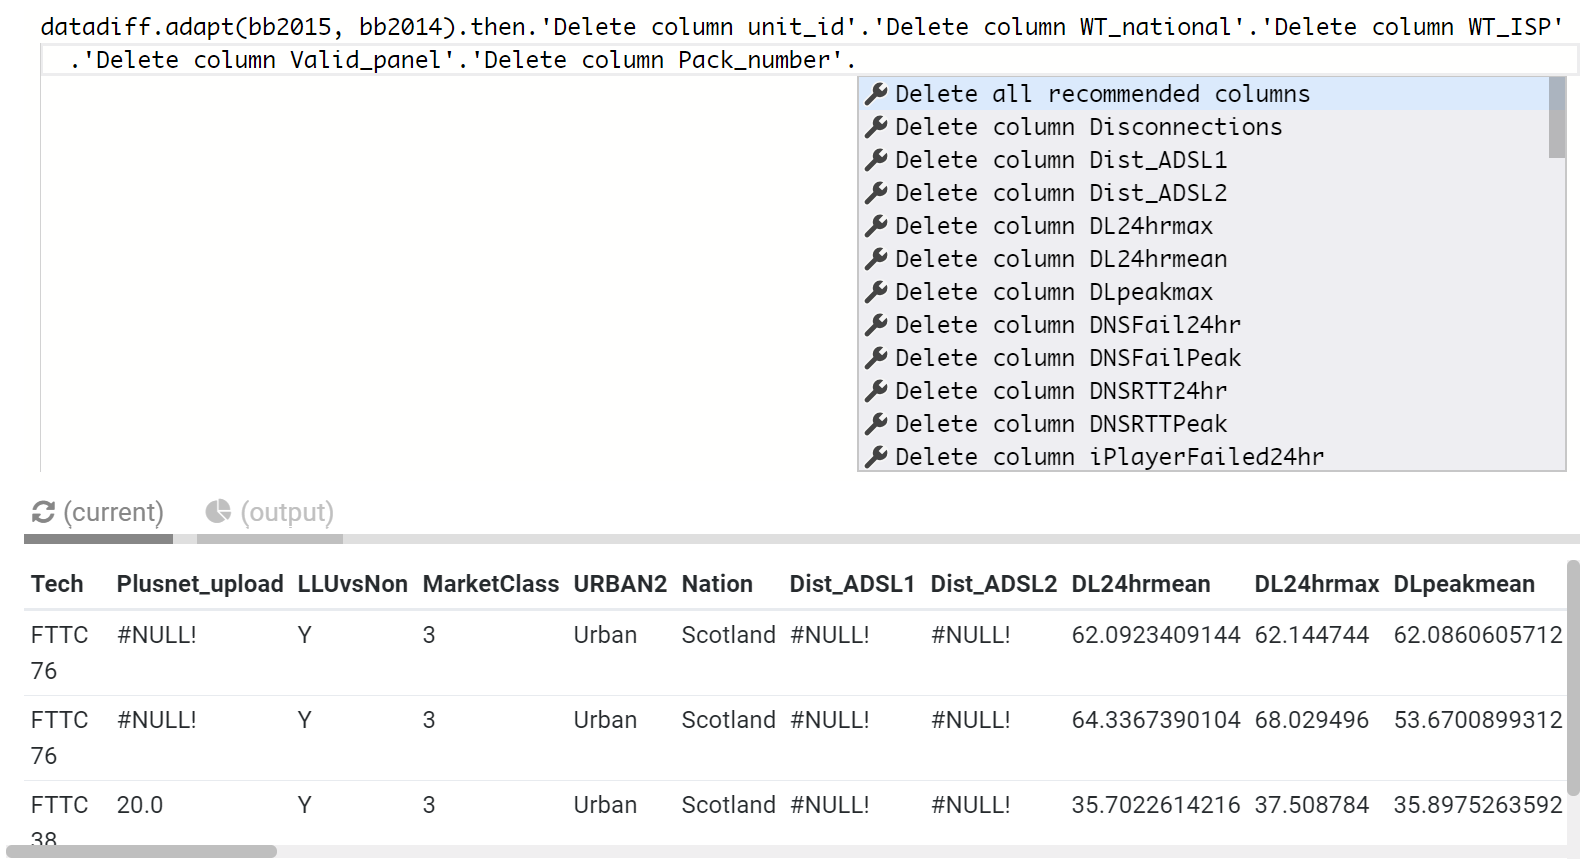
\includegraphics[scale=0.29]{wrattler.png}
\caption{The datadiff AI assistant running inside Wrattler, a notebook-like environment for
data science. The completion list shows data cleaning operations offered by an AI assistant 
and the preview shows the result of running the provided cleaning script.}
\label{fig:wrattler}
\end{figure}

\section{AI assistants in a notebook environment}
\label{sec:notebook}

Before looking at the formal model which aims to explain what an AI assistant is, it is useful 
to explore how AI assistants can be used in a notebook programming environment for data science 
such as Jupyter. Figure~\ref{fig:wrattler} shows a screenshot of a datadiff AI assistant, running
in the Wrattler notebook system.

In the example, a user obtained two datasets, \texttt{bb2015} and \texttt{bb2014} that contain 
information about broadband speeds for years 2015 and 2014. The two data sets record observations
over two years, containing a common subset of data, but in a mismatched format -- the column names
and order differ. The data analyst invokes the datadiff AI 
assistant in order to turn the format of 2015 data into the format used by the 2014 dataset.
To do this, they type \texttt{datadiff.adapt(bb2015, bb2014)}, which invokes the AI assistant.
They then type ``.'' to get a data cleaning recommendation.

The AI assistant analyses the data and determines a list of patches that needs to be applied in
order to reformat the 2015 dataset. It then offers those patches in the autocompletion list, 
sorted from the most likely patch to the least likely patch. The user can proceed by selecting 
the first patch repeatedly (as in the above screenshot). After selecting a patch, the source code
in the cell changes and the preview is updated, showing the result of running the current cleaning
script. This interactivity makes it easy to see possible data cleaning errors. If applying a patch
does not lead to an expected result, the user can easily go back and select the second most likely
patch.

Modelling an AI assistant as a tree, we can see that the code entered in the editor corresponds to
a path through the tree (where the user provides information for the AI asistant; here, by 
accepting some of the recommended patches). The options shown in an auto-complete list correspond 
to the possible sub-trees in the current tree node (here, the AI assistant is asking for an user 
input or a recommendation on how to continue). 


\section{Formal model of AI assistants}
\label{sec:trees}

An AI assistant is a concept that spans multiple research areas. In order to understand how to 
integrate AI assistants into programming tools such as notebooks, we need to use methods from 
programming language research. To implement interesting AI assistants, we need to use machine 
learning and statistical models.

From a programming language perspective, we are mainly interested in the abstract structure of the
AI assistant. A programming langauge model will capture how data is passed to the assistant, how
is the assistant invoked and how does it interact with the analyst. From a machine learning
perspective, we are interested in how to build AI assistants. For example, many assistants may fit
in the Bayesian learning model where the AI assistant updates an initial model -- a prior --
based on inputs from the analyst. 

\tpnote{It would be nice to have more about Bayesian model of AI assistants - but I'm not qualified
to write that. We'd need to show how a Bayesian model defines ``AI assistant as a tree structure'' 
(probably quite easy) and give some Bayesian AI assistant examples... (could be quite simple, but
we don't have them)}
However, it is conceivable that an AI assistant can be implemented in other ways. It might provide
suggestions based on a simple frequentist statistical analysis, or it might use models based on 
neural networks. The programming language model of what is an AI assistant should be able to 
accommodate all those different implementations. Modelling AI assistants as trees, as discussed
in the next section, satisfies this requirement as it allows a range of different concrete
implementations.

\subsection{Programming abstraction: AI assistants as trees}
\label{sec:trees-def}

To discuss properties of AI assistants from a programming language perspective, we model an AI 
assistant as a function that takes some input data and generates a tree where each node offers a 
finite list of options that the user can choose from. For simplicity, we ignore the possibility of 
open-ended options where the user specifies some input and we also ignore the fact that the AI 
assistant might take some initial parameters in addition to the input. Assuming \ident{Data}
is a representation of input data:
%
\begin{equation*}
\begin{array}{rcll}
a &=& \ident{Data} \rightarrow t &\textnormal{(AI assistant)}\\
t &=& (n_1, r_1, e_k, t_1), \ldots (n_k, r_k, e_k, t_k) &\textnormal{(Provided options)}\\
\mathit{eval} &=& \ident{Data}\times e \rightarrow \ident{Data}&\textnormal{(Evaluator for the DSL)}
\end{array}
\end{equation*}
%
An AI assistant $a$ is a function that takes some input data and returns a root tree node~$t$. 
A tree node consists of a list of branches $(n_i, r_i, e_i, t_i)$ where $n_i$ is a name of the branch 
(shown to the user, but otherwise unimportant), $r_i$ is a number that gives a rating of the option
(between 0 and 1), $e_i$ is an expression in the domain-specific language that represents
the data transformation attached to the node. Finally, $t_i$ is a sub-tree that can be empty or can 
offer more follow-up options. Note that this sub-tree can be generated lazily -- it is only needed 
if the user chooses the option with which it is associated and so we do not need to evaluate the 
full tree upfront.

The nature of expressions $e$ depends on the particular AI assistant and so we leave that abstract
for now. However, we certainly need to be able to apply the transformation on sample dataset. 
This is captured by the $\mathit{eval}$ function, which takes data together with an expression $e$
in the domain-specific langauge and returns transformed data. 

\newpage

\begin{figure}
\hspace{4em}\begin{forest}, tt  
  [
    [{$\mathbf{n_1}$\\$p=0.9$\\$e=e_1$}
      [{$\quad\mathbf{n_{11}}\quad$\\$r=0.9$\\$e=e_{11}$}]
      [{$\quad\mathbf{n_{12}}\quad$\\$r=0.7$\\$e=e_{12}$}]
    ]
    [{$\mathbf{n_2}$\\$p=0.8$\\$e=e_2$}
      [{$\quad\mathbf{n_{21}}\quad$\\$r=0.9$\\$e=e_{21}$}]
      [{$\quad\mathbf{n_{22}}\quad$\\$r=0.8$\\$e=e_{22}$}]
    ]
    [{$\mathbf{n_3}$\\$p=0.7$\\$e=e_3$}
      [{$\quad\mathbf{n_{31}}\quad$\\$r=0.8$\\$e=e_{31}$}]
      [{$\quad\mathbf{n_{32}}\quad$\\$r=0.6$\\$e=e_{32}$}]
    ]
  ]
\end{forest}
\caption{An illustration of a formal model that views AI assistants as trees.}
\label{fig:aitree}
\vspace{-1em}
\end{figure}

\noindent
Figure~\ref{fig:aitree} illustrates the formal model and shows an (abstract) example of a tree
that can be generated by an AI assistant. The root node offers three options represented by nodes 
$n_1, n_2, n_3$. The most likely one as recommended by the AI assistant is $n_1$ with rating $r=0.9$. 
The expression attached to the node is $e_1$ and when the user selects the node, we can display a 
preview using sample data $\mathit{sample}$ using the $\mathit{eval}$ function by evaluating 
$\mathit{eval}(\mathit{sample}, e_1)$.

Assuming the user chooses the most likely option $n_1$, they will then be presented with two
subsequent options, $n_{11}, n_{12}$. Even though the AI assistant marks the first node as more
likely, the user may review the previews $\mathit{eval}(\mathit{sample}, e_{11})$,
$\mathit{eval}(\mathit{sample}, e_{12})$ and decide that the latter is actually the correct
data cleaning operation. They can then choose the node $n_{12}$ as the final one use the 
cleaning script represented by the DSL expression $e_{12}$. The expression $e_{12}$ can be used
to get the clean data by evaluating $\mathit{eval}(\mathit{sample}, e_{12})$, but it can also be
translated to a programming language such as R or Python and used in a larger data wrangling 
workflow.

\section{Examples of AI assistants}
\label{sec:examples}

\tpnote{The examples here illustrate the idea, but are not detailed enough for a proper paper
(we should also have only the better version of datadiff). It would be ideal to have CSV, better
datadiff and some Bayesian example. Possibly also ptype, but it might not fit the model that well --
we need to think about that.}

We now consider two AI assistants through the lens of our abstract tree model.
The first is hypothetical AI assistant for extracting data from CSV files. The second
is the datadiff assistant. For datadiff, we discuss the current implementation in Wrattler, but
also briefly sketch a possible improvement (that improves the interactivity aspect).

\subsection{Cleaning CSV files}

\tpnote{This is inspired by Gerrit's work, but it's very basic at this point.}
  
As an example, consider the following broken CSV file. The file starts with two meta-data lines
(one specifying the name and another specifying copyright information). This is followed by headers
and actual data.

\begin{Verbatim}[numbers=left,xleftmargin=8mm]
Counts of things
Copyright (c) Poor data export company, London, UK
Name, City, Count
Joe, London, 3
Jane, Edinburgh, 16
Jim, Cardiff, na
\end{Verbatim}

A minimalistic AI assistant for cleaning CSV files generates tree with two levels of nodes. 
In the first level, it infers where the actual data is in the CSV file (and it offers 
its best guesses to the user). In the second level, it infers the types of the columns. 

The domain-specific language for CSV parsing consists of just two functions named
$\ident{range}$ and $\ident{types}$ that specify the range of data in the file and the types
of the columns: $\ident{range}(\ident{lines}=l_n\ldots l_m, \ident{cols}=k)$ denotes that
the data starts on line $l_n$ and ends on line $l_m$ and there are $k$ columns; 
$\ident{types}(t_1,\ldots, t_k)$ specifies that the types of the $k$ columns are 
$t_1, \ldots, t_k$. The types are either $\ident{string}$ or $\ident{int}$.

\begin{figure}
\begin{equation*}
\begin{array}{l}
r=0.9,~ e=\ident{range}(\ident{lines}=2\ldots 6, \ident{cols}=3)\\[0.2em]
\qquad\longrightarrow r=0.9,~ e=\ident{range}(\ident{lines}=2\ldots 6, \ident{cols}=3); \ident{types}(\ident{string},\ident{string},\ident{string})\\[0.2em]
\qquad\longrightarrow r=0.3,~ e=\ident{range}(\ident{lines}=2\ldots 6, \ident{cols}=3); \ident{types}(\ident{string},\ident{string},\ident{int})\\[0.4em]
r=0.7,~ e=\ident{range}(\ident{lines}=3\ldots 6, \ident{cols}=3)\\[0.2em]
\qquad\longrightarrow r=0.8,~ e=\ident{range}(\ident{lines}=3\ldots 6, \ident{cols}=3); \ident{types}(\ident{string},\ident{string},\ident{int})\\[0.2em]
\qquad\longrightarrow r=0.7,~ e=\ident{range}(\ident{lines}=3\ldots 6, \ident{cols}=3); \ident{types}(\ident{string},\ident{string},\ident{string})\\[0.4em]
r=0.3,~ e=\ident{range}(\ident{lines}=1\ldots 6, \ident{cols}=1)\\[0.2em]
\qquad\longrightarrow r=0.9,~ e=\ident{range}(\ident{lines}=1\ldots 6, \ident{cols}=1); \ident{types}(\ident{string})\\[0.2em]
\end{array}
\end{equation*}
\caption{A tree generated by an AI assistant for parsing CSV files. Each node has a rating $r$ and
a data cleaning expression $e$ written in a small domain-specific language for cleaning CSV files.}
\label{fig:csvtree}
\end{figure}

Given the above CSV file as an input, the AI assistant produces a tree shown in Figure~\ref{fig:csvtree}.
At the first level, the AI assistant gives us three options. The first, most likely, one skips just 
the first line and identifies that there are three columns (this error is made because the second line contains 
two commas and can thus be interpreted as data row). The second option skips first two lines and recognises
three columns. The AI assistant might find this less likely, but it is the option we want to choose
as users. Finally, the third option takes all lines, but then it has to join all columns into one
which is unlikely.

The user can choose the second option, at which point a user interface can evaluate the 
expression $\ident{range}(\ident{lines}=3\ldots 6, \ident{cols}=3)$ and show a preview of 
the cleaning result as a parsed table, but without types. Next, the user has a choice of two ways of inferring types -- the most 
likely one (and the right one) is that the third column has a type \ident{int} (which means that
the value {\texttt na} in the last row will be treated as missing). If {\texttt na} was not 
representing a missing value, the user could choose the second option which infers the type of the 
last column as \ident{string}.

The resulting expression 
$\ident{range}(\ident{lines}=3\ldots 6, \ident{cols}=3); \ident{types}(\ident{string},\ident{string},\ident{int})$
can then be applied to the input data using the $\mathit{eval}$ function, which gives us 
columns \ident{Name} of type \ident{string}, \ident{City} of type \ident{string}
and \ident{Count} of type \ident{int} with data:
%
\begin{equation*}
\begin{array}{l}
(\textnormal{\sffamily "\hspace{-0.2em}Joe"}, \textnormal{\sffamily "\hspace{-0.2em}London"}, 3)\\
(\textnormal{\sffamily "\hspace{-0.2em}Jane"}, \textnormal{\sffamily "\hspace{-0.2em}Edinburgh"}, 16)\\
(\textnormal{\sffamily "\hspace{-0.2em}Jim"}, \textnormal{\sffamily "\hspace{-0.2em}Cardiff\hspace{0.1em}"}, \mathit{NaN})
\end{array}
\end{equation*}

\subsection{Current design of datadiff AI assistant}

\tpnote{I describe current version of datadiff first and then a possible improvement. If we turn
this into a paper, we should have just one (preferably the latter) version. This section might
be useful for the AIDA team though.}
The datadiff package takes two tabular datasets that are in inconsistent formats, but represent
two sets of observations about the same entity. An example is measurements of broadband speed in
two different yers, stored as two tabular files with missing or additional columns, using different
order of columns and different column names.

Datadiff generates a list of patches that can be applied to one dataset in order to convert it to the
format used by the second dataset. The patches form a domain-specific language (DSL) of the 
data transformation suggested by datadiff. A patch $p$ can be one of the following:
%
\begin{equation*}
\begin{array}{lcll}
p &=& \ident{permute}(\pi) &\textnormal{(Reorder columns using a given permutation)}\\
  &|& \ident{recode}(i, [s_1\mapsto s_2, \ldots]) &\textnormal{(Recode categorical values using in column $i$)}\\
  &|& \ident{linear}(i, a, b)&\textnormal{(Apply linear transform $va+b$ to a numerical column $i$)}\\
  &|& \ident{delete}(i)&\textnormal{(Drop the column at index $i$)}\\
  &|& \ident{insert}(i, d)&\textnormal{(Insert a new column at index $i$ initialized to values $d$)}
\end{array}
\end{equation*}
%
The current implementation of datadiff is a non-interactive R package that takes two datasets
and produces a list of patches. It takes a couple of parameters that specify which patches should
datadiff attempt to generate (together with various weights to tweak the optimization).

The current datadiff AI assistant as implemnented in Wrattler generates a tree that allows the
user to select and apply individual patches. The user can review each patch to make sure that it
is a reasonable transformation. For example, consider the following two datasets:

\vspace{0.5em}
\begin{minipage}[t]{0.5\textwidth}
\begin{Verbatim}[numbers=left,xleftmargin=3mm]
Name, City
Joe, London
Jane, Edinburgh
Jim, London
\end{Verbatim}
\end{minipage}
\begin{minipage}[t]{0.5\textwidth}
\begin{Verbatim}[numbers=left,xleftmargin=3mm]
City, Name, Count
Cardiff, Alice, 1
Cardiff, Bob, na
Edinburgh, Bill, 2
\end{Verbatim}
\end{minipage}
\vspace{1em}

\noindent
If we ask datadiff for a list of patches to transform the dataset on the right-hand side
to the format of the dataset on the left-hand side, we might get the following patches
(assuming columns are indexed from $1$):
%
\[
\ident{delete}(3);~ \ident{permute}(2,1);~ \ident{recode}(2, [\textnormal{\sffamily "\hspace{-0.2em}Cardiff\hspace{0.1em}"}\mapsto\textnormal{\sffamily "\hspace{-0.2em}London"}])
\]

\noindent
Datadiff correctly infers that we need to drop the newly added {\ttfamily Count} column and that
the order of {\ttfamily Name} and {\ttfamily City} has been switched. It might also suggest that
{\ttfamily City} is a categorical column where the encoding has been changed, which is not the 
case here (but this would be a reasonable guess if one dataset contained values ``true'' and ``false''
while the other contained ``yes'' and ``no'').

\begin{figure}
\begin{equation*}
\begin{array}{l}
r=0.9,~ e=\ident{delete}(\ldots)\\[0.2em]
\qquad\longrightarrow r=0.9,~ \ident{delete}(\ldots); \ident{permute}(\ldots)\\[0.2em]
\qquad\qquad\longrightarrow r=0.6,~ \ident{delete}(\ldots); \ident{permute}(\ldots); \ident{recode}(\ldots)\\[0.2em]
\qquad\longrightarrow r=0.6,~ \ident{delete}(\ldots); \ident{recode}(\ldots)\\[0.2em]
\qquad\qquad\longrightarrow r=0.9,~ \ident{delete}(\ldots); \ident{recode}(\ldots); \ident{permute}(\ldots)\\[0.4em]
r=0.8,~ e=\ident{permute}(\ldots)\\[0.2em]
\qquad\longrightarrow r=0.9,~ \ident{permute}(\ldots); \ident{delete}(\ldots)\\[0.2em]
\qquad\qquad\longrightarrow r=0.6,~ \ident{permute}(\ldots); \ident{delete}(\ldots); \ident{recode}(\ldots)\\[0.2em]
\qquad\longrightarrow r=0.6,~ \ident{permute}(\ldots); \ident{recode}(\ldots)\\[0.2em]
\qquad\qquad\longrightarrow r=0.9,~ \ident{permute}(\ldots); \ident{recode}(\ldots); \ident{delete}(\ldots)\\[0.4em]
(\ldots)
\end{array}
\end{equation*}
\caption{A tree generated by a basic datadiff AI assistant. The parameters of the patches are
omitted -- they are the same as in the full list of patches shown above. }
\label{fig:ddtree}
\end{figure}

The tree generated by the datadiff AI assistant based on the three inferred patches is shown 
in Figure~\ref{fig:ddtree}.
At the first level, the user can choose one of the three patches (we only show sub-trees for the first two). 
The patches are sorted by their rating and so \ident{delete} is offered before \ident{permute}. In the
second level, the user can choose one of the remaining patches. Assuming the user follows the first
branch and chooses \ident{delete}, they can now choose to apply \ident{permute} or \ident{recode} (the
first option being more likely). In the last third level, the AI assistant offers the remaining patch. 
The user can stop before reaching the leaf and choose just $\ident{delete}(3);~ \ident{permute}(2,1)$ 
as the final data cleaning script, ignoring the \ident{recode} patch. 

This example shows why AI assistants provide a more convenient developer interface. The \ident{recode}
patch would, in some cases, be a reasonable data cleaning recommendation, but a human analyst can
look at the values and see that this is not the case here. (We could imagine an assistant that
integrates semantic information into the process and recognizes that the values represent cities.
This solves the specific problem shown here, but leaves many similar problems unsolved.) When using
datadiff as a cleaning function in R, we would get all three patches, apply them and then (hopefully)
notice the incorrect recoding. We could fix the result by tweaking the parameters of the function,
e.g.~by lowering the threshold for \ident{recode} patches. When using an AI assistant, the analyst
can review all patches instantly and skip the unsuitable ones. 

As before, the data wrangling expressions can be evaluated using the \emph{eval} function (to get 
previews when writing the code in a notebook environment), but they can also be translated to 
simple R or Python scripts for production use.

\subsection{Alternative design of datadiff AI assistant}
\label{sec:examples-datadiff2}

\tpnote{Again, we should have just one version, preferably this one. Can we somehow formulate
this as a Bayesian model -- i.e. we have some prior that is updated based on the choices that
a user makes? If so, that would be neat.}

The current design of the datadiff AI assistant is not optimal, because it performs a global
optimization up-front and then merely allows the user to choose some of the patches. This is 
problematic, because the global optimization can be slow (so the initial step might take too
much time) and the result of the optimization does not improve based on the user input.

For example, if the user could specify that a certain column should not be recoded, datadiff 
could run an optimization taking this constraint into account and, say, match columns differently 
(this is currently not possible, because the current version runs the global optimization once 
up-front and then merely offers a choice of produced patches).

A better datadiff AI assistant would generate expressions in the same domain-specific 
language as the current one (list of patches $p$). However, the tree would be generated and 
structured differently. This could be done by maintaining a list of constraints and generating
the best possible patch given certain constraints, together with a choice of most likely constraints
the user might want to add. A constraint $c$ is defined as:
%
\begin{equation*}
\begin{array}{lcll}
c &=& \ident{norecode}(i) &\textnormal{(Values in a categorical column $i$ should not be recoded)}\\
  &|& \ident{notransform}(i)&\textnormal{(Values in a numerical column $i$ should not be transformed)}\\
  &|& \ident{nodelete}(i)&\textnormal{(Column $i$ should not be deleted)}\\
  &|& \ident{match}(i,j)&\textnormal{(Column $i$ should be mapped to sample column $j$)}
\end{array}
\end{equation*}
%
The first three constraints specify that certain patches should not be generated. The last one is
more interesting as it allows the user to explicitly give a mapping for a column (but unless other
constraints are given, datadiff can still attempt to transform or recode the column to get a 
better match). This is likely not a complete set of constraints, but it is sufficient to illustrate
the idea.

The AI assistant would then implement a function that takes two datasets together with a set of 
constraints and generates a cleaning script together with a list of constraints (sorted by their
ranking) that the user might want to add. (If we allowed nodes with open-ended options, the
user could write an arbitrary constraint, but for now, we just assume that the AI assistant can
generate all sensible options.)

Using the above function, we can produce a tree as follows. We start with an empty set of 
constraints $C=\{\}$ and call the function to obtain a data cleaning DSL expression $e$ and
potential constraints $c_1, \ldots, c_k$. For each constraint, we add it to the set $C$ and
generate a sub-tree by calling the AI assistant function recursively. In other words, following
a path through the tree would add more and more constraints to the set $C$ and each node will
come with the best DSL expression that datadiff can generate under the constraints determined
by the path taken through the tree. The following illustrates (a small part of) the tree that 
the revised AI assistant for datadiff would generate for the above two files. (In addition to a DSL 
expression $e$ and rangking $r$, we also include a set of constriants $C$ associated with each 
node):
%
\begin{equation*}
\begin{array}{l}
C=[], r=1,~ e=\ident{delete}(\ldots);~ \ident{permute}(\ldots);~ \ident{recode}(\ldots)\\
\qquad\longrightarrow C=[\ident{norecode}(2)], r=0.4, e=\ident{delete}(\ldots);~ \ident{permute}(\ldots);\\
\qquad\qquad\longrightarrow C=[\ident{norecode}(2); \ident{nodelete}(3)], p=0.2, e=(\ldots)\\
\qquad\qquad\longrightarrow (\ldots)\\
\qquad\longrightarrow C=[\ident{nodelete}(3)], r=0.2, e=\ident{delete}(\ldots);~ \ident{permute}(\ldots);~ \ident{recode}(\ldots)\\
\qquad\longrightarrow C=[\ident{match}(1,1)], r=0.4, e=\ident{delete}(\ldots);~ \ident{permute}(\ldots);~ \ident{recode}(\ldots)\\
\qquad\longrightarrow C=[\ident{match}(1,2)], r=0.8, e=\ident{delete}(\ldots);~ \ident{permute}(\ldots);~ \ident{recode}(\ldots)\\
\qquad\longrightarrow (\ldots)
\end{array}
\end{equation*}
%
The tree has only one root node which was generated without any constraints. The generated expression
is the best guess by datadiff, which drops the {\texttt Count} column, rearranges columns and recodes
(incorrectly) the {\texttt City} column. The nodes at the second level allow the user to add a
number of constraints. 

\newpage
The first two sub-nodes prevent datadiff from generating two patches that it employed. The first one
disallows recoding the column {\texttt City}. The resulting expression drops {\texttt Count} and
rearranges the columns, which is the result we were hoping to obtain. 
The second sub-node disallows deleting the {\texttt Count} node. In this case, datadiff has to
find other ways of reconcilling the data sets, perhaps by recoding {\texttt Code} and dropping
another column. Finally, the last two sub-nodes allow us to explicitly specify a mapping between
columns. The listing only shows the first two (map column $1$ to column $1$; map column $1$ to column $2$),
but the AI assistant can generate the full list.

\section{Evaluating AI assistants}
\label{sec:evaluation}

\tpnote{This section has only notes on ``methods for evaluating AI assistants in general'' but it 
does not actually do any concrete evaluation of specific AI assistants using those general methods.
We'll obviously need to add that in a real paper (once we have concrete AI assistants we want to 
talk about).}

Evaluating AI assistants is hard, because they are not fully automatic. They are designed to 
assist a human data analyst in solving a data wrangling problem. We could evaluate the experience 
of using an AI assistant on a sample task using a user study. This would be no doubt worthwhile, 
but it would assess the user experience rather than the quality of the artifical intelligence 
methods employed by an AI assistant. In this section, we consider how to evaluate whether an 
AI assistant provides good data wrangling suggestions to the data analyst. 

The fact that all AI assistants follow a common framework -- i.e. they can be viewed as trees with
ranked branches and data wrangling scripts in each node -- means that we can discuss evaluation 
methods that can be used to assess the quality of any AI assistant, rather than inventing a 
suitable evaluation method individually for each assistant. The most important aspect of such
evaluation methods is how they account for the interactivity of AI assistants. Before discussing
this, we first consider how can a fully automatic data wrangling function be evaluated.

\subsection{Evaluating fully automatic cleaning functions}
\label{sec:eval-auto}

\tpnote{This is somewhat long methodological comment. It may be useful for the AIDA team, but
perhaps not so much for a real paper (perhaps if it was a bit shorter).}
We first consider how to evaluate an AI data wrangling tool that is implemented as a simple 
function -- the data analyst calls it on input data and it produces clean data as an output.
There are several ways in which such function can be evaluated:
%
\begin{itemize}
\item \textbf{Sample benchmarks.} If we have a collection of sample inputs with clean outputs,
  we can assess how close the outputs produced by the tool are to the clean outputs. This method
  relies on having an extensive benchmark for each particular problem, which is rarely the case.
\item \textbf{Corruption patches.} We can generate input/output pairs by taking 
  a number of clean datasets (as the outputs) and corrupting them by introducing
  annomalies which the automatic tool should then detect and remove. This evaluation method requires 
  less manual work, but it is limited by how realistict the corruption patches are (i.e.~we only
  test the tool on problems that we can easily imagine).
\item \textbf{Statistical analysis.} In some cases, there might be a way to generate inputs 
  semi-randomly, run the cleaning tool and then use some statistical property of the input/output
  pair to assess the tool. This can be done when there is a statistical property that is easy
  to check, but finding the transformation is hard.
\end{itemize}

\subsection{Evaluating interactive AI assistant}

Evaluating AI assistants is more complicated than evaluating automatic functions.
AI assistants do not just produce one output -- they organise possible outputs in a tree with 
ranked branches and we should evaluate how good the tree is overall. The following three 
sections consider different aspects of the tree that could be evaluated.

\subsubsection{Evaluating AI assistant as an automatic tool}

First of all, we can treat an AI assistant as a fully automatic tool. To do this, we automatically
choose the most likely option provided by the AI assistant until we reach a leaf node or
until we reach a node where all the branches have ranking below a certain threshold (e.g.~$r\leq 0.5$).

More formally, given a dataset $d$ and an AI assistant $a$ (as defined in Section~\ref{sec:trees-def}), 
we run the AI assistant $a(d)$ to obtain a list of options $(n_1, r_1, e_k, t_1), \ldots (n_k, r_k, e_k, t_k)$.
We choose the most likely node $(n_i, r_i, e_i, t_i)$ (i.e. $r_i \geq r_j$ for all $j$). If 
$t_i$ is empty or the ranking of all options inside $t_i$ are less than a given threshold, we return
an expression $e_i$; otherwise, we recursively follow the sub-tree $t_i$. Finally, we evaluate
the resulting data cleaning expression using $\mathit{eval}(d, e_i)$ to get the clean output for
the input data $d$.

Now that we have an input/output pair, we can evaluate how good the cleaned data set is using 
methods for evaluating automatic cleaning functions discussed in the previous section (either 
by running the assistant on a benchmark, or by generating a benchmark using corrpution patches).
This way, we can guarantee that the interactive AI assistant is as good as an automatic cleaning 
function would be. This is a reasonable baseline test, but it does not tell us much about how
good the interactive aspects are.

\subsubsection{Evaluating interactivity of AI assistants}

One of the motivations for the idea of AI assistants was that real-world data cleaning tasks
often have ad-hoc issues that require some form of manual intervention. In other words, the 
file might have an annomaly that a human can spot, but that an automatic data cleaning algorithm
would miss. For example, consider the following two CSV files:

\vspace{0.5em}
\begin{minipage}[t]{0.5\textwidth}
\begin{Verbatim}[numbers=left,xleftmargin=3mm]
Name, Count, ID
Jim, 45, 1
Jane, 52, 2
Joe, 67, 3
\end{Verbatim}
\end{minipage}
\begin{minipage}[t]{0.5\textwidth}
\begin{Verbatim}[numbers=left,xleftmargin=3mm]
Name, Code, Value
Alice, 35, 4
Bill, 38, 5
Bob, 42, 6
\end{Verbatim}
\end{minipage}
\vspace{0.5em}

\noindent
As humans, we can look at the column names and guess that the column {\texttt ID} should be 
aligned with {\texttt Code} and {\texttt Count} should likely match {\texttt Value}. However, 
unless the AI assistant ``understands English'', it has no way of discovering this. 

\paragraph{Hidden anomalies.}
We say that a \emph{hidden anomaly} is a value in the data set that has statistical properties
compatible with the rest of the values, but does not fit among the other values in some other
sense -- which typically relies on human understanding of the value or on additional semantic
information. The definition is likely always going to depend on a particular AI assistant -- we
can continue improving AI assistant to detect more and more hidden anomalies, but there will always
be cases that require human insigth. That said, there are some typical examples of hidden anomalies.

Examples of hidden anomalies might include rows that are not outliers in the statistical sense
(such as the row in a CSV file containing copyright information, but having correct number of commas), 
textual values that have the right format, but wrong meaning (such as ``Refugee Olympic Athletes'' 
among the names of countries\footnote{This is a name for an actual team of 10 athletes competing 
in the 2016 Rio Olympic games.}), or a suspicious numerical value such as $123.45678$ in a numerical 
column with values $190.52136, 58.68297, 123.45678, 67.47067, 47.69846$.

Following the idea of ``corruption patches'' introduced when discussing the evaluation of automatic
data wrangling tools (Section~\ref{sec:eval-auto}), it might be possible to produce a set of common
hidden anomalies and write scripts that will corrupt a clean data set and also introduce hidden 
anomalies during the process. However, it is not clear whether this can be done in general, or
whether this needs to be done case-by-case for each particular AI assistant.

\paragraph{Eliminating hidden anomalies interactively.}
Hidden anomalies are problems in data that cannot be detected and removed by a fully automatic
data wrangling tool (i.e.~a tool that is implemented as a function). An important quality of AI 
assistants is that they should make it possible to eliminate hidden anomalies with a small 
number of interactions, ideally just by choosing an appropriate non-default offered option at one 
point when traversing the tree. For example, given the above example, the alternative datadiff AI 
assistant would allow us to choose a tree node that adds a constraint $\ident{match}(2,3)$ and 
we would get the correct result with just one manual intervention (the other column would be 
reordered automatically).

To summarise, we want to be able to claim that an AI assistant makes it easy to handle ad-hoc
corner cases that are not discovered by the machine learning algorithm behind it. To do this,
we introduce hidden anomalies into the data -- those are plausible real-world data annomalies 
that are not discovered by the algorithm emplyed by the AI assistant. A good AI assistant allows
the user to eliminate these with a minimal number of interactions, i.e.~choices of other than
the most likely nodes in the tree. 

\subsubsection{Easy discoverability of best results}

Finally, the current integration for AI assistants in Wrattler exposes the tree through a
user interface. The user calls the AI assistant and then chooses a sub-tree to explore 
(by typing `.' and choosing one of the options in a drop-down menu). This means that it is
desirable to make the most likely result (domain-specific language expression) closer to the
root rather than somewhere deep in the tree.

As an example, consider the two designs of the datadiff assistant. In the first design, the
user has to manually accept all the desired patches. If the optimal patch needs to drop 15
extra columns from a dataset, the user will have to make 15 choices explicitly. The
second design of the datadiff assistant is better because the most likely set of patches
is available immediately in the root node (and users only need to continue exploring a
sub-tree if they need to address an hidden annomaly).

\begin{figure}
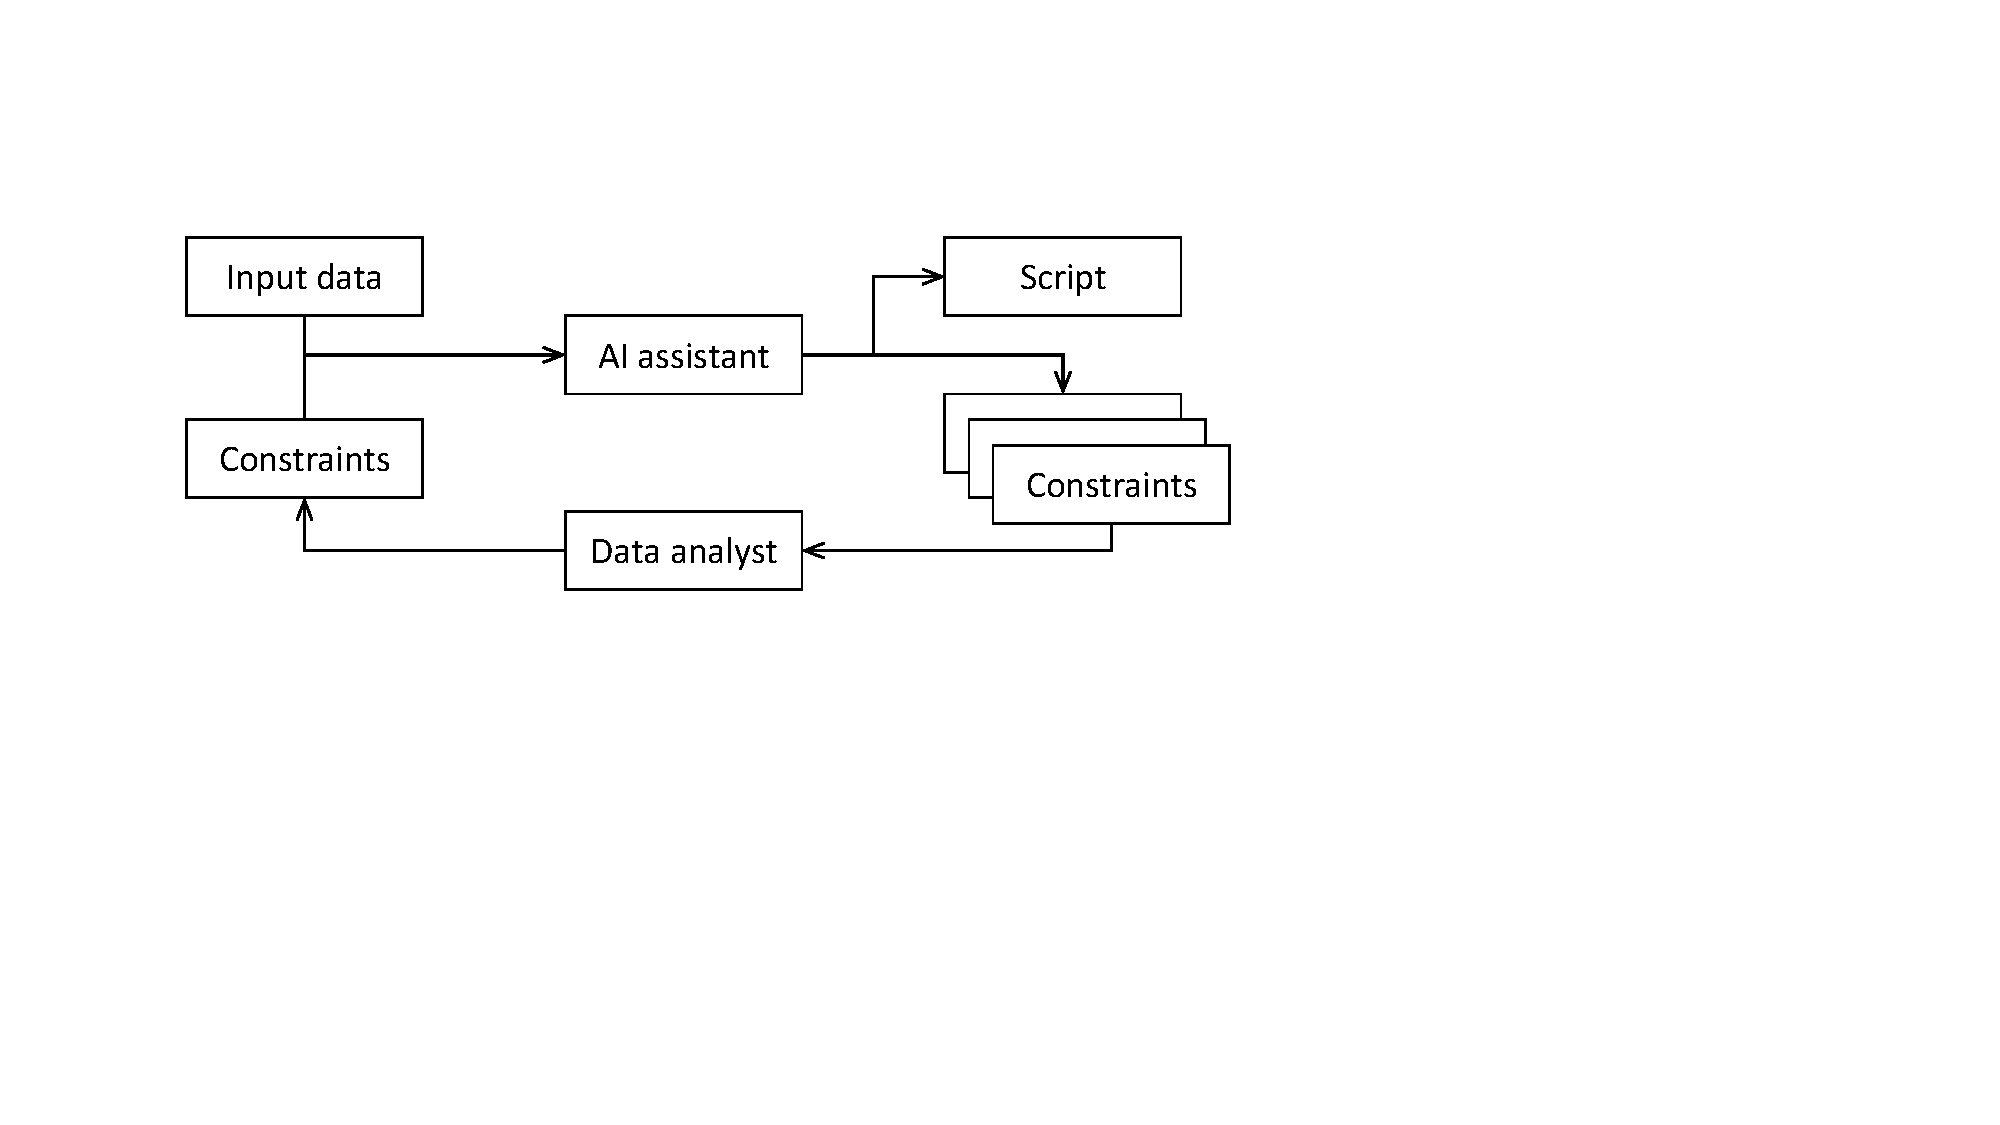
\includegraphics[scale=0.55,trim=1cm 8.5cm 11cmm 4cm,crop]{diagrams.pdf}
\caption{Information flow in an adaptive AI assistant based on collecting constraints.}
\label{fig:aiflow}
\end{figure}

\section{Further work and open questions}
The formal model and examples presented in this document are very basic, but they capture the
main idea of ``what is an AI assistant''. We focused on the simplest possible model of 
interaction -- choosing one from several options, modelled as selecting one branch from a tree.
This has obvious limitations. It does not allow the data analyst to give free form feedback 
to the AI assistant. However, this model can be nicely integrated with developer tools (via 
auto-complete) and still captures a wide range of useful AI assistants. Considering more general
models would be an interesting follow-up work, but this paper focuses on taking the first step.

\tpnote{For a proper paper, I think we need to write more about the constraints/Bayesian model,
but we can leave composing of AI assistants as future work.}

In this section, we discuss two other directions for future work. First, we consider one way in
which many AI assistants could be built. Second, we consider ways of composing multiple AI 
assistants.

\subsection{Adaptive AI assistants}
One pattern that seems particularly useful when implementing AI assistants is using constraints
as discussed in the second version of datadiff assistant (Section~\ref{sec:examples-datadiff2}).
In this case, we implement a function that takes a set of constraints and produces the best 
possible data wrangling script for given data under given constraints. The function also needs
to provide possible constraints that could reasonably be added to the set. Given such function,
we can build an AI assistant that creates a tree -- nodes correspond to sets of constraints and
branches correspond to adding constraints to the set. 

The idea of an AI assistant that is generated based on constraints is illustrated in 
Figure~\ref{fig:aiflow}. The AI assistant is invoked on the input data with an initial set of
constraints (typically empty). It produces a data wrangling script (best recommendation under
the given constraints) together with a set of constraints that it suggests to the data anlyst.
The analyst either accepts the script, or chooses one of the constraints and adds it to the
list of constraints for the AI assistant. The assistant then makes another suggestion and the
loop continues.

Not all AI assistants can be implemented in this way, but it is a useful common pattern that is
worth developing in more detail. There are a number of open questions.

\paragraph{Bayesian interpretation.}
The idea of having initial set of constraints and then adapting the result of a machine learning
algorithm based on input from the user sounds closely related to Bayesian machine learning. In 
that case, we start with some prior assumptions about data. We can then run a machine learning 
algorithm to make predictions about the data based on those assumptions. However, we then adapt
the model based on new observations.

\tpnote{I'm writing this, but I don't know what I'm saying! I just hope that someone from the AIDA 
team can correct this and write something more interesting :-)}

In case of AI assistants, the prior would be either some automatically generated ``best guess''
and the new observations used to adapt the model would be the inputs (or choices) specified by 
the data analyst. The first question is, what is the relationship of this idea to the approach
based on constraints -- are these two just two different ways of saying the same thing, is one
of the methods more general than the other, or are they just two unrelated useful patterns?

\tpnote{These are just random thoughts -- but I think we can only answer this if we actually 
try building some example concrete AI assistant based on the Bayesian idea -- and then we'll
see how it actually needs to work. It would be great if we did this!}
The second question is what is needed in order to better support the Bayesian model of AI assistants.
Would the data analyst need to specify some initial input to the AI assistant? And what are the
ways in which the additional data might be specified? In our current model, the AI assistant has
to provide a range of options to choose from. Is this flexible enough for an AI assistant based
on a Bayesian model, or do we need a more flexible form of interaction, for example one where the
data analyst can input some data manually as examples?

\paragraph{Specifying initial parameters.} 
In the case of datadiff, we started with an empty set of constraints. However, in some cases, it
might be desirable to provide more input to the AI assistant before using it. Such input could 
include an initial set of constraints (in a format akin to that used by the revised version of 
datadiff) or information about a Bayesian prior. For example, the user might want to specify 
assumptions about relationships between columns in a CSV file (in order to help an AI assistant
that attempts to fill missing values based on values from related columns).
\tpnote{The idea about column relationships might be useful for the work Alfredo is doing.}

Yet another interesting example would be AI assistants that take a probabilistic model as an 
input. This might be a simple description of a model or a more complex one such as a function
written in a probabilistic programming language. Such AI assistant could then interactively
work with the user on either refining the program, or inferring best parameters. Alternatively,
the AI assistant could be used as an interactive mechanism for constructing a probabilistic 
program -- it might start with an empty program and then provide a way for adding different 
program logic to it.
\tpnote{Again, this is just wild speculation -- we'd need a concrete example to say more about
this, but I quite like the idea...}


\subsection{Composing multiple assistants}

As discussed earlier, AI assistants are designed to solve one particular data wrangling task and
we expect that a data analyst will typically need to interact with several AI assistants during 
the data wrangling process. In this document, we assume that this will be done manually and that
the AI assistants will be invoked manually, one after another, to solve specific tasks. This 
might be sufficient if the tasks are distinct (e.g.~scraping data from the web, merging data
sets, identifying outliers, etc.), but it is also worth considering how to best integrate multiple 
AI assistants.

\tpnote{This is all fairly speculative, but I wanted to record all ideas that we discussed!}

\paragraph{Combining assistants.}
When the user loads a messy data set, they might not initially know how to get started cleaning
it. They have a variety of AI assistants available, but it might still be difficult to know
where to start. One way of integrating AI assistants that would be useful in this scenario is
creating a ``meta-AI assistant'' that advises the user what AI assistants to apply and in which
order. This could be, perhaps, done by looking at the rankings of choices reported by the AI
assistants and finding the ones that are the most certain about their results.

\paragraph{Sharing information between assistants.}

It might be also desirable to have a more fine grained way of integrating AI assistants. For
example, say we have two separate AI assistants; one for parsing CSV files and an one for inferring
types from data. Ideally, we would be able to interleave the uses of these two, so that the CSV
assistant finds data in the text file and the type inferrence assistant then infers the type
of the data. The information about the quality of the inferred types could then be fed back to the
CSV assistant (which might use it as a measure of how well it identified the data in the file).

This level of interaction is not currently possible, because there is no way of exchanging 
information between AI assistants. There are two possible directions we could investigate. 
First, it might be possible for multiple adaptive assistants based on constraints to share the 
wrangling domain specific langauge and constraints language. We could then invoke multiple
assistants in the data cleaning loop as shown in Figure~\ref{fig:aiflow}. 

Alternatively, the AI assistants could communicate by attaching more semantic information to 
the data (or, generating scripts that attach semantic information to the data). If the input 
data was not just a data frame with raw values, but a table with additional semantic information,
one assistant could recover some semantic information and another assistant could then use it.
For example, we might run type inferrence assistant first (to annotate data with likely types).
If we then invoked datadiff, it could use these inferred types to better match columns from 
multiple data files.
\end{document}
























%